\documentclass[12pt]{article}
\usepackage{fullpage,enumitem,amsmath,amssymb,graphicx,grffile,float,listings}



\begin{document}
    %Title Section
    \begin{flushleft}
	\LARGE Braitenberg Vehicles
    \end{flushleft} 
    \rule{\linewidth}{0.4pt}
    %Title Section

    %Problem and Solution

    \section*{Simulating a Braitenberg Vehicle}

	Consider the braitenberg vehicle, a vehicle with wheels that spin in proportion to their respective sensor reading.

	\begin{figure}[h]
		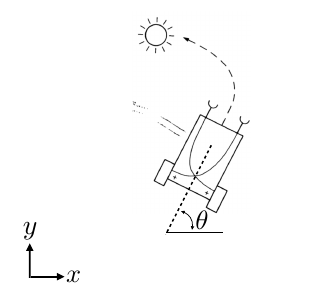
\includegraphics[width=8cm]{./figure1.png}
		\centering
		\caption{Braitenberg vehicle.}
	\end{figure}

	\noindent The state of the robot consists of its position and orientation and can be modeled as \newline $q = \begin{bmatrix} x & y & \theta \end{bmatrix}^T$.
	Let $v$ be the speed of the robot. We can model the state of the robot as it evolves over time as:
	\begin{equation}
		\pmb{\dot q} = \begin{bmatrix} v\cos{\theta} \\ v\sin{\theta} \\ \dot{\theta} \end{bmatrix}
	\end{equation}

	The flow of information through our system is modeled as follows:

	\begin{figure}[H]
		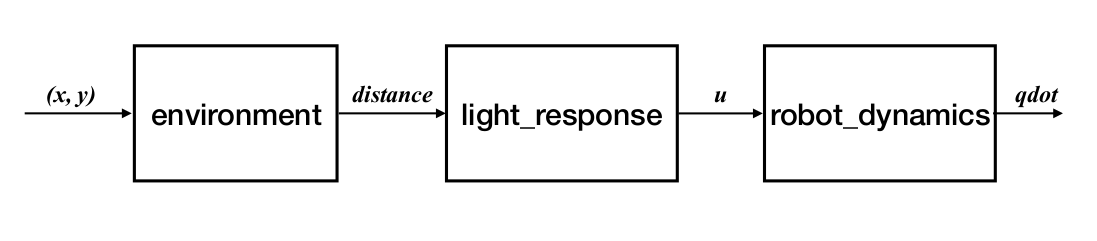
\includegraphics[width=14cm]{./figure2.png}
		\centering
		\caption{Braitenburg System.}
	\end{figure}

	The system input is $\pmb{u} = \begin{bmatrix} v, \dot \theta \end{bmatrix}^T$. The robot dynamics can be simulated using the following functions: 
	
	\begin{itemize}
		\item \texttt{robot\_dynamics}: simulate system dynamics, $\pmb{\dot q}$.
		\item \texttt{environment}: compute the distance from a light source to the robot's sensors.
		\item \texttt{light\_response}: compute wheel velocities from light sensor readings.
	\end{itemize}

	Three versions, \emph{coward}, \emph{aggresive}, and \emph{instincts}, of \texttt{light\_response}, have been implemented below.


\end{document}
